\section{Strategy for Finding Minimal Obstructions} \label{sec:strategy}

In this section, we describe the general strategy to show that every non-extendible partial
representation contains one of the obstructions described in
Section~\ref{sec:definition_of_obstructions}. 

For any two disjoint subtrees $T_i$ and $T_j$ of the MPQ-tree $T$, we write $T_i \wlt T_j$ if and
only if there exist cliques $a \in T_i$ and $b \in T_j$ such that $a \wlt b$. In this situation, the
maximal cliques of $T_i$ are forced to appear on the left of the maximal cliques of $T_j$.

\heading{Testing Extendibility by MPQ-tree Reordering.}
Recall that a MPQ-tree $T$ represents all feasible orderings of the maximal cliques of a given
interval graph $G$. By Lemma~\ref{lem:repext_char}, a partial representation is extendible if and
only if there exists a reordering $T'$ of $T$ such that the frontier of $T'$ extends $\wlt$. This
condition can be tested by the following algorithm (see~\cite{kkosv}).

We process the MPQ-tree $T$ from the bottom to the root. When a P-node is processed, we test whether
there exists a linear extension of $\wlt$ on its subtrees. It exists if and only if $\wlt$ induced
on the subtrees of the node is acyclic. Thus, if there is a cycle, the MPQ-tree cannot be reordered
according to $\wlt$. When a Q-node is processed, there are two possible orderings of its subtrees,
and we check whether any of them is compatible with $\wlt$. The partial representation is extendible
if and only if all nodes can be reordered in this manner. See Fig.~\ref{fig:reordering_example} for
an example. 

\begin{figure}[b!]
\centering
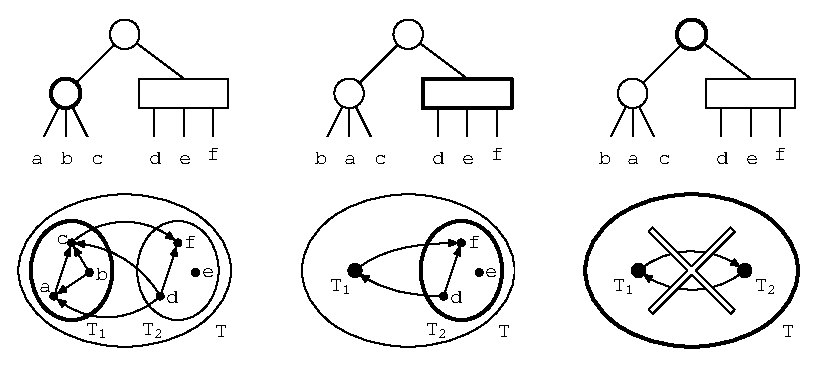
\includegraphics{strategy_reordering_example.eps}
\caption[]{This example is from~\cite{kkosv}, and it shows from left to right the way in which the reordering
algorithm works. We depict comparable pairs of maximal cliques by directed edges. The processed
trees are contracted into vertices.

\hskip 1em First, we reorder the highlighted P-node on the left. The subdigraph induced by $a$, $b$
and $c$ is ordered $b \rightarrow a \rightarrow c$. We contract this subtree $T_1$ into a vertex.
Next, we keep the order of the highlighted Q-node and contract its subtree $T_2$ into a vertex. When
we reorder the root P-node, the algorithm finds a two-cycle between $T_1$ and $T_2$, and outputs
``no''.}
\label{fig:reordering_example}
\end{figure}

%\begin{lemma}[\cite{kkosv}] \label{lem:reordering_testing}
%A partial representation is extendible if and only if the MPQ-tree can be reordered according to
%$\wlt$. The above algorithm tests this correctly.
%\end{lemma}

A node that cannot be reordered is called \emph{obstructed}. A set of maximal cliques
\emph{creates} an obstruction if the ordering of this set in $\wlt$ makes the node
obstructed.

\heading{Strategy.} Suppose that a partial representation $\calR'$ is non-extendible.
From~\cite{kkosv}, we know that there exists an obstructed node in the MPQ-tree. We divide the
argument into three cases, according to the type of this node: \emph{an obstructed leaf}
(Section~\ref{sec:leaves}), \emph{an obstructed P-node} (Section~\ref{sec:p_nodes}), and \emph{an
obstructed Q-node} (Section~\ref{sec:q_nodes}).  Figure~\ref{fig:diagram} shows an overview of the
proof.

\begin{figure}[t!]
\centering
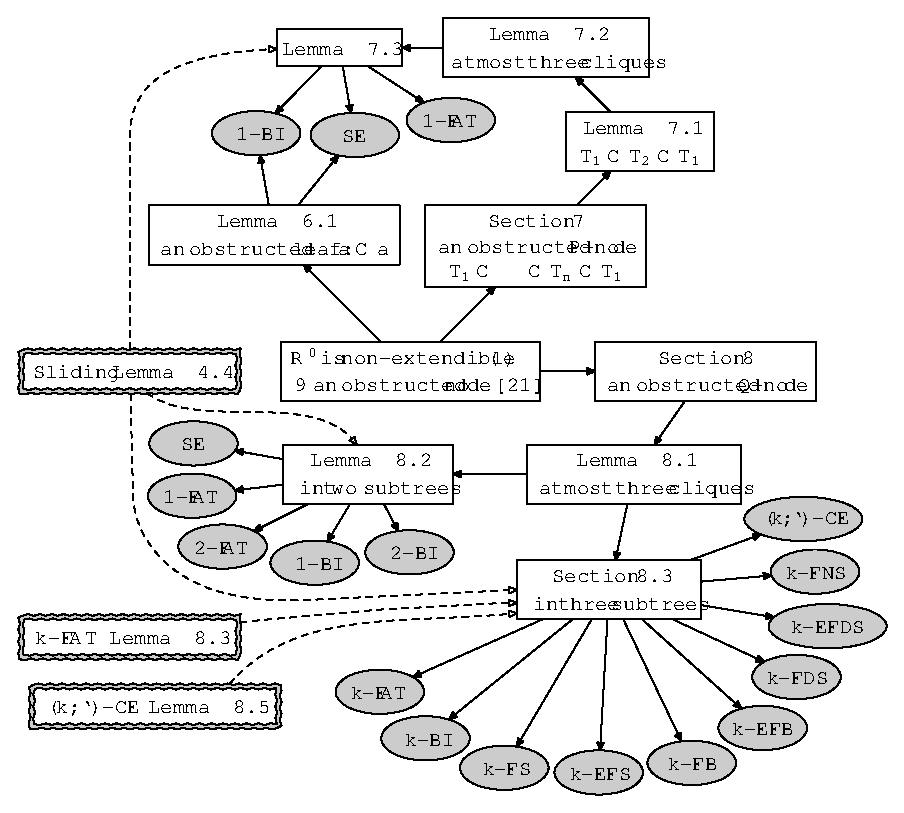
\includegraphics{strategy_diagram.eps}
\caption{Overview of the main steps of the proof, it starts in the middle. The obtained
obstructions are highlighted in gray, and three tools are depicted with highlighted borders. The
most involved case is in Section~\ref{sec:q_nodes_three_subtrees}.}
\label{fig:diagram}
\end{figure}

First, we argue that there exist at most three maximal cliques creating an obstruction.
Then, we consider their positions in the MPQ-tree and their open intervals from the definition of
$\wlt$. We use tools of Sections~\ref{sec:maximal_cliques} and~\ref{sec:interval_orders} to derive
positions of several pre-drawn intervals forming one of the obstructions.

In Section~\ref{sec:q_nodes_k_fat}, we prove a key tool called $k$-FAT Lemma~\ref{lem:k_fat}:
If three non-adjacent vertices $x_k$, $y_k$, and $z_k$ are pre-drawn in an order that is
different from their order in the sections of a Q-node, then they induce a $k$-FAT obstruction.
The proof is done by induction for $k$, and it explains why complicated obstructions are
needed.
